\documentclass{beamer} % blue; brown; gray; red;
\usepackage{beamerthemesplit}
\usepackage{beamerthemeshadow}
\usepackage{animate}
\usepackage[3D]{movie15}
\usepackage{hyperref}
%\usepackage[numbered]{mcode}
\usepackage{graphics}
\usepackage{pgf,pgfarrows,pgfnodes,pgfautomata,pgfheaps}
\usepackage{amsmath,amssymb}
\usepackage{pgfpages}
%\setbeameroption{show only notes}
%\setbeameroption{show notes on second screen=right}
\usepackage{tikz}
\usetikzlibrary{trees}
\usetikzlibrary{decorations.pathmorphing}
\usetikzlibrary{decorations.markings}


\usetheme{Warsaw}

\usecolortheme{sidebartab}
%beetle,crane,dove,fly,seagull,wolverine,beaver
\renewcommand{\raggedright}{\leftskip=0pt \rightskip=0pt plus 0cm}
\raggedright
\graphicspath{{figures/}}
\definecolor{MyDarkGreen}{rgb}{0.0,0.4,0.0}


%%%%%%%%%%%%%%%%%%%%%%%%%%%%%%%%%%%%%%%%%%%%%%%%%%%%%%
\usepackage{xeCJK}
\usepackage{fontspec}
\setCJKmainfont[BoldFont=simhei.ttf]{simkai.ttf}
%\setCJKsansfont{simhei.ttf}
%\setCJKmonofont{simfang.ttf}

%%%%%%%%%%%%%%%%%%%%%%%%%%%%%%%%%%%%%%%%%%%%%%%%%%%%%%%%%%%%%%%%%%%%%%%%%%
\makeatletter
\usefoottemplate{ %重新定义页脚,加入作者,单位,单位图标,和文档标题
  \vbox{\tiny%
    \hbox{%
      \setbox\beamer@linebox=\hbox to\paperwidth{%
        \hbox to.5\paperwidth{
            \hfill\tiny\color{white}
                  \textbf{\insertshortauthor\quad\insertshortinstitute}
            \hskip .1cm\lower 0.2em\hbox{
\includegraphics[height=0.25cm]{./figures/CAS.pdf}}
            \hskip.3cm}%
        \hbox to.5\paperwidth{
            \hskip.3cm\tiny\color{white}
                  \textbf{\insertshorttitle}\hfill}\hfill}%
      \ht\beamer@linebox=2.625ex%
      \dp\beamer@linebox=0pt%
      \setbox\beamer@linebox=\vbox{\box\beamer@linebox\vskip1.125ex}%
      \color{structure}\hskip-\Gm@lmargin\vrule width.5\paperwidth
      height\ht\beamer@linebox\color{structure!70}\vrule width.5\paperwidth
      height\ht\beamer@linebox\hskip-\paperwidth%
      \hbox{\box\beamer@linebox\hfill}\hfill\hskip-\Gm@rmargin}
  }
}
\makeatother
%%%%%%%%%%%%%%%%%%%%%%%%%%%%%%%%%%%%%%%%%%%%%%%%%%%%%%%%%%%%%%%%%%%%%%%%%%

\begin{document}

\title{DPD方法及其它无网格方法的边界条件}
\subtitle{组会}
\author[周吕文]{周吕文}


\institute[中国科学院力学研究所,LHO]{中国科学院力学研究所,LHO}
\date{2011年03月14日}
\subject{Computer Tools, TeX, Slide}

%%%%%%%%%%%%%%%%%%%%%%%%%%%%%%%%%%%%%%%%%%%%%%%%%%%%%%%%%%%%%%%%%%%%%%%%%%
\frame[plain]{
\titlepage
} % 产生主题页,plain选项表示不显示页眉页脚等内容


\titlegraphic{\pgfuseimage{title}}
\AtBeginSection[]{ % 在每个Section前都会加入的Frame
  \frame<handout:0>{
    \frametitle{Outline}
    \tableofcontents[current,currentsubsection]
  }
}



\section{边界类型}
\frame{\frametitle{边界类型}

对于所有的计算流体力学问题,边界条件都是重要的研究内容。在无网格方法中,一般有以下几类边界条件:

\begin{itemize}
\item 周期边界
\item 粒子层法
\item 粒子反弹运动方法

\begin{enumerate}
\item 镜子映像(Specular reflection)
\item 反弹映像(bounce-back reflection)
\item 麦克斯韦映像(Maxwellian reflection)
\end{enumerate}

\item 粒子层与反弹运动方法结合
\end{itemize}

}

\subsection{粒子层法}
\frame{\frametitle{粒子反弹运动方法}

粒子反弹运动方法:(a)镜子映像(Specular reflection); (b)反弹映像(bounce-back reflection); (c)麦克斯韦映像(Maxwellian reflection)

\begin{columns}
\begin{column}[c]{0.25\textwidth}
\begin{center}
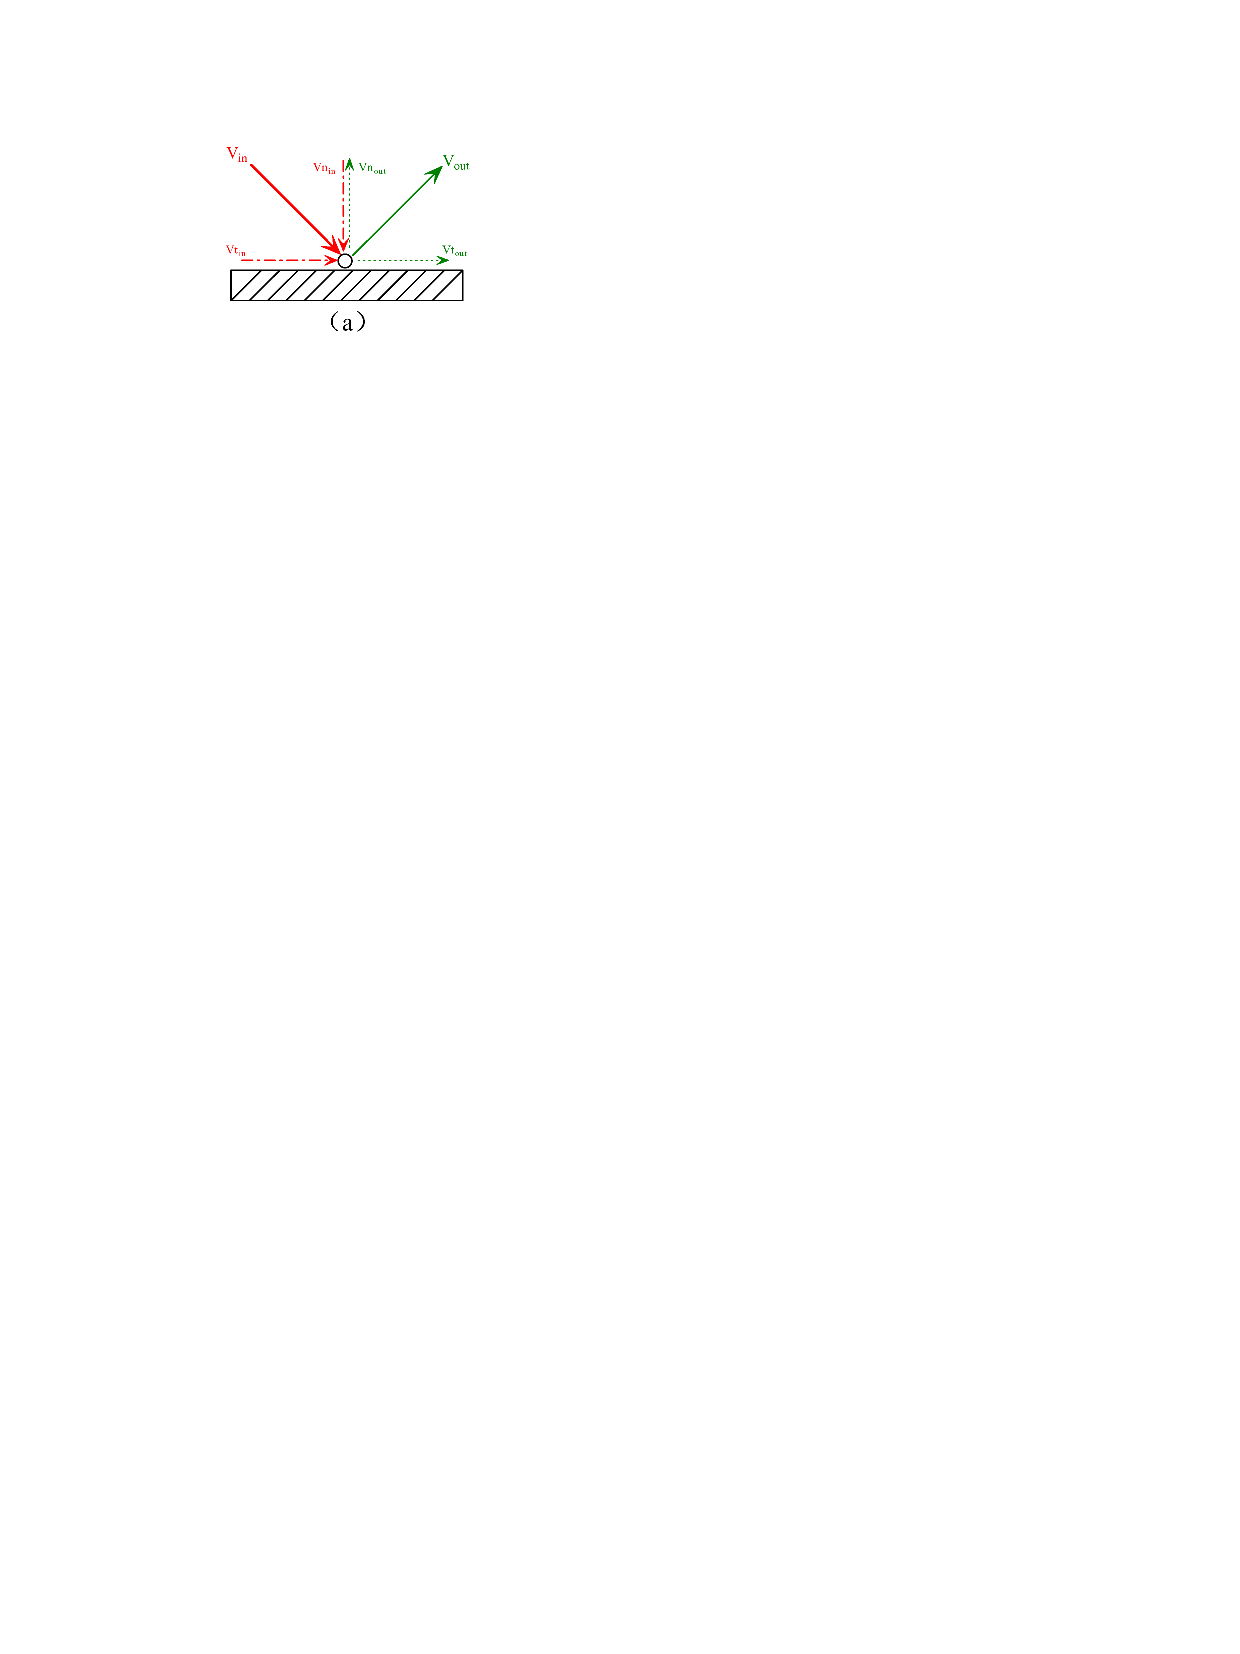
\includegraphics[width=1\textwidth]{./figures/fig02_1.pdf}
\end{center}
\end{column}
\begin{column}[c]{0.25\textwidth}
\begin{center}
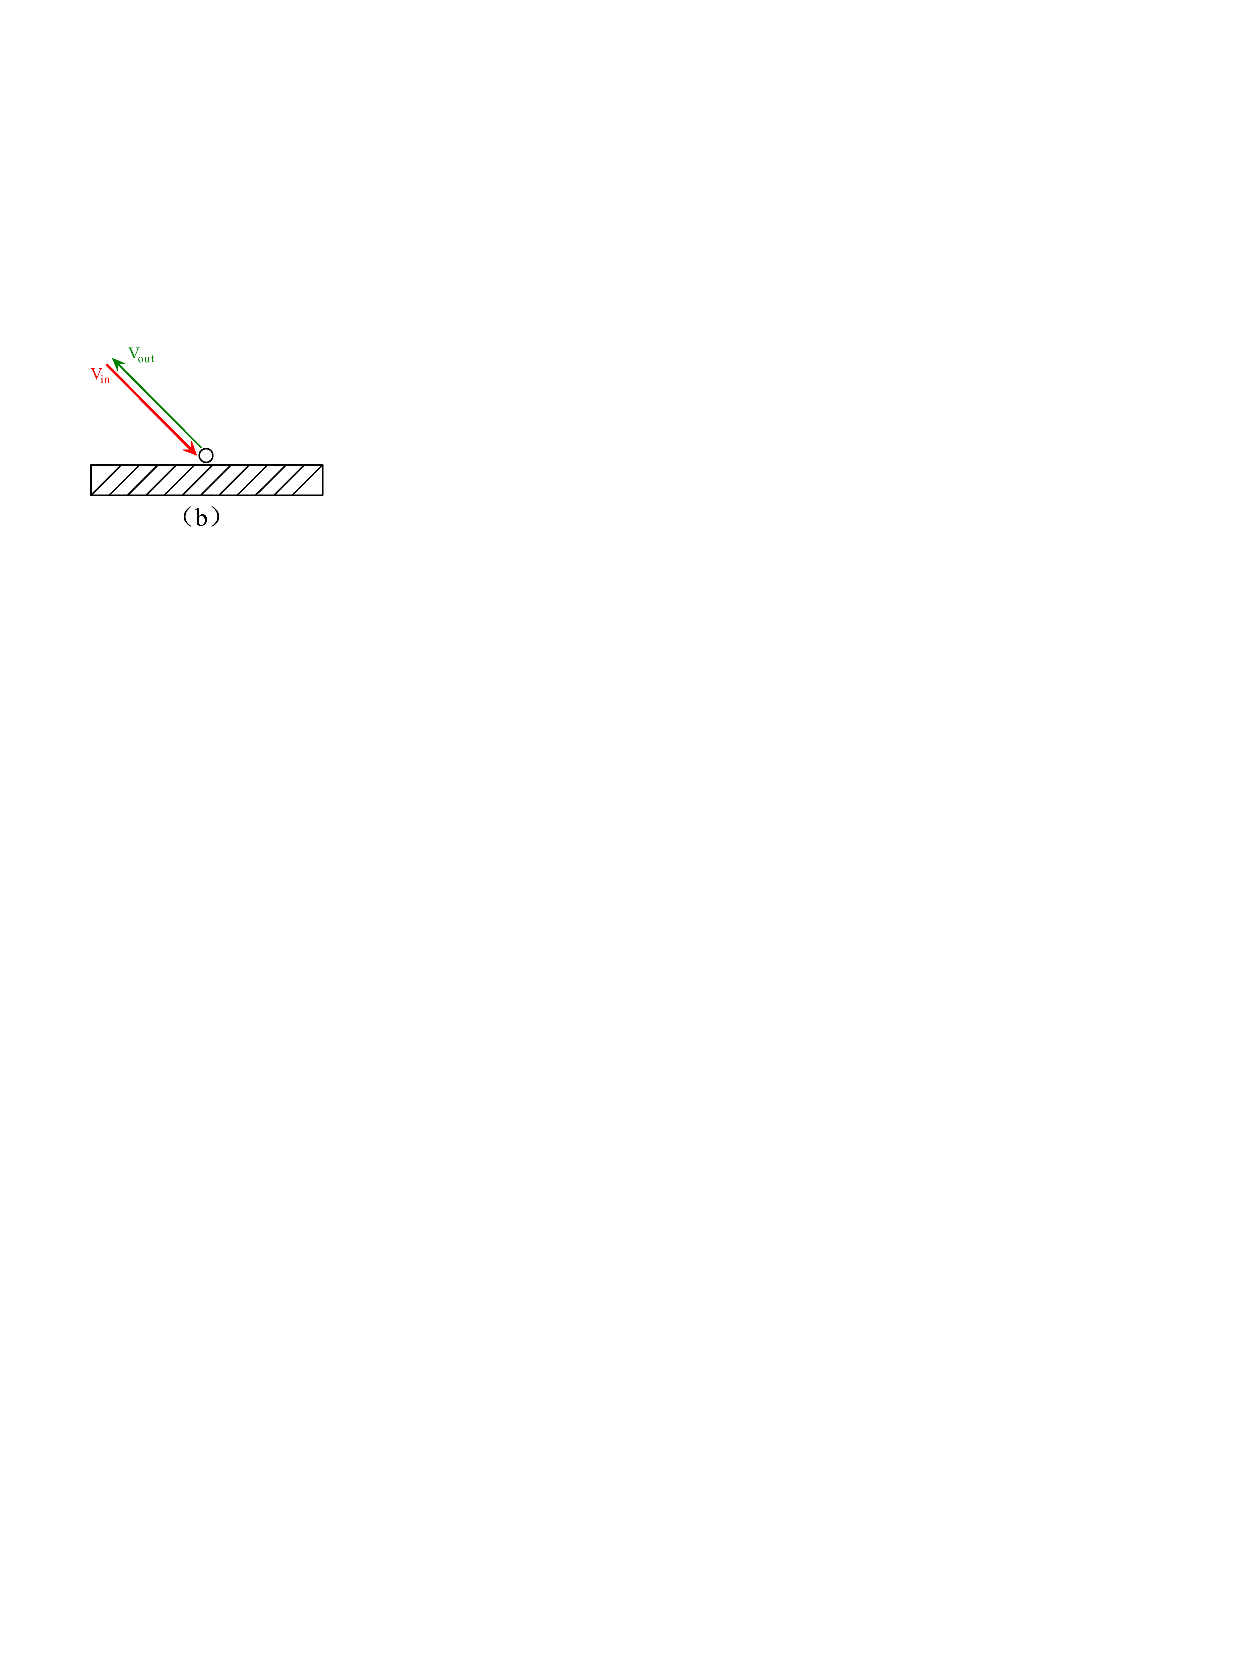
\includegraphics[width=1\textwidth]{./figures/fig02_2.pdf}
\end{center}
\end{column}
\begin{column}[c]{0.25\textwidth}
\begin{center}
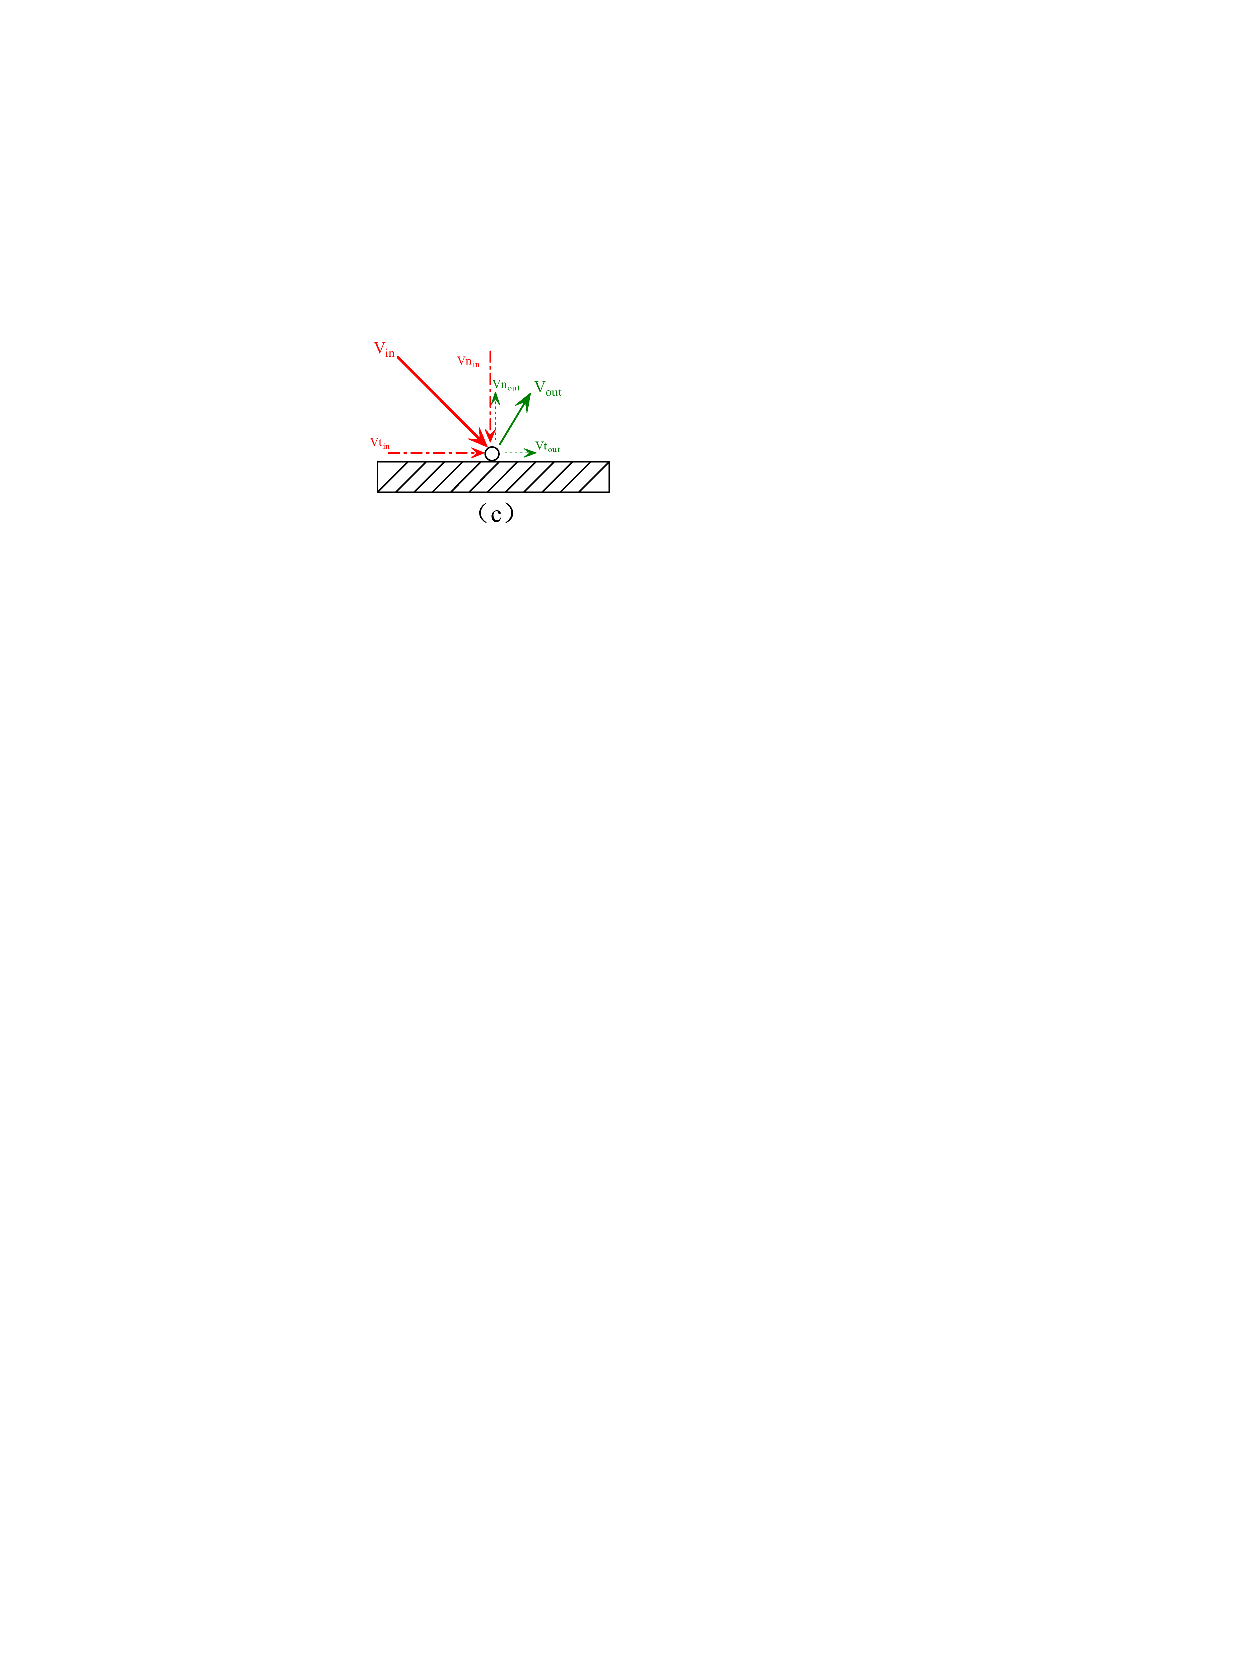
\includegraphics[width=1\textwidth]{./figures/fig02_3.pdf}
\end{center}
\end{column}
\end{columns}
}

\subsection{粒子层与反弹运动方法结合}

\frame{\frametitle{粒子层与反弹运动方法结合}

粒子层与反弹运动方法结合

\begin{center}
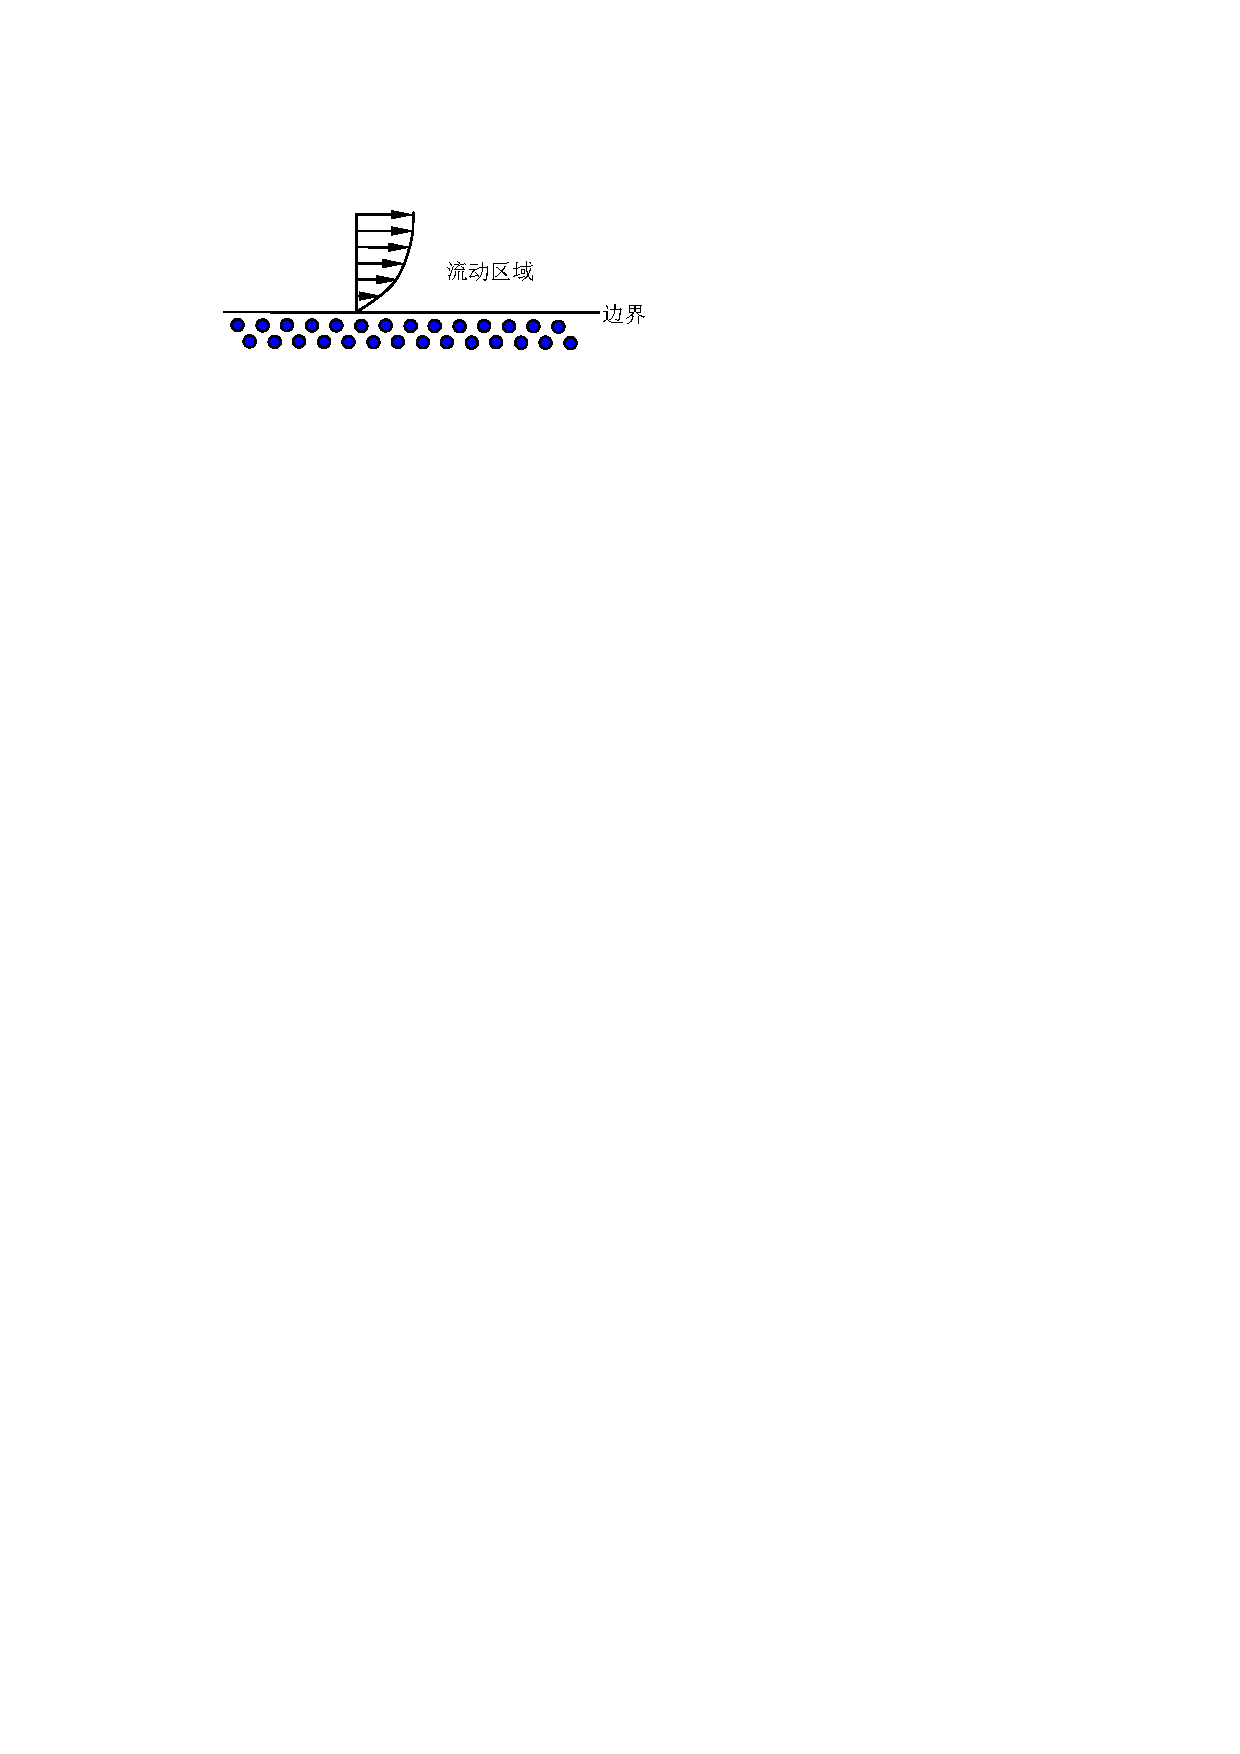
\includegraphics[width=0.7\textwidth]{./figures/fig03.pdf}
\end{center}

}


\section{Boundary condition in dissipative particle dynamics}


\subsection{模型}
\frame{\frametitle{模型}
\begin{columns}
\begin{column}[c]{0.4\textwidth}
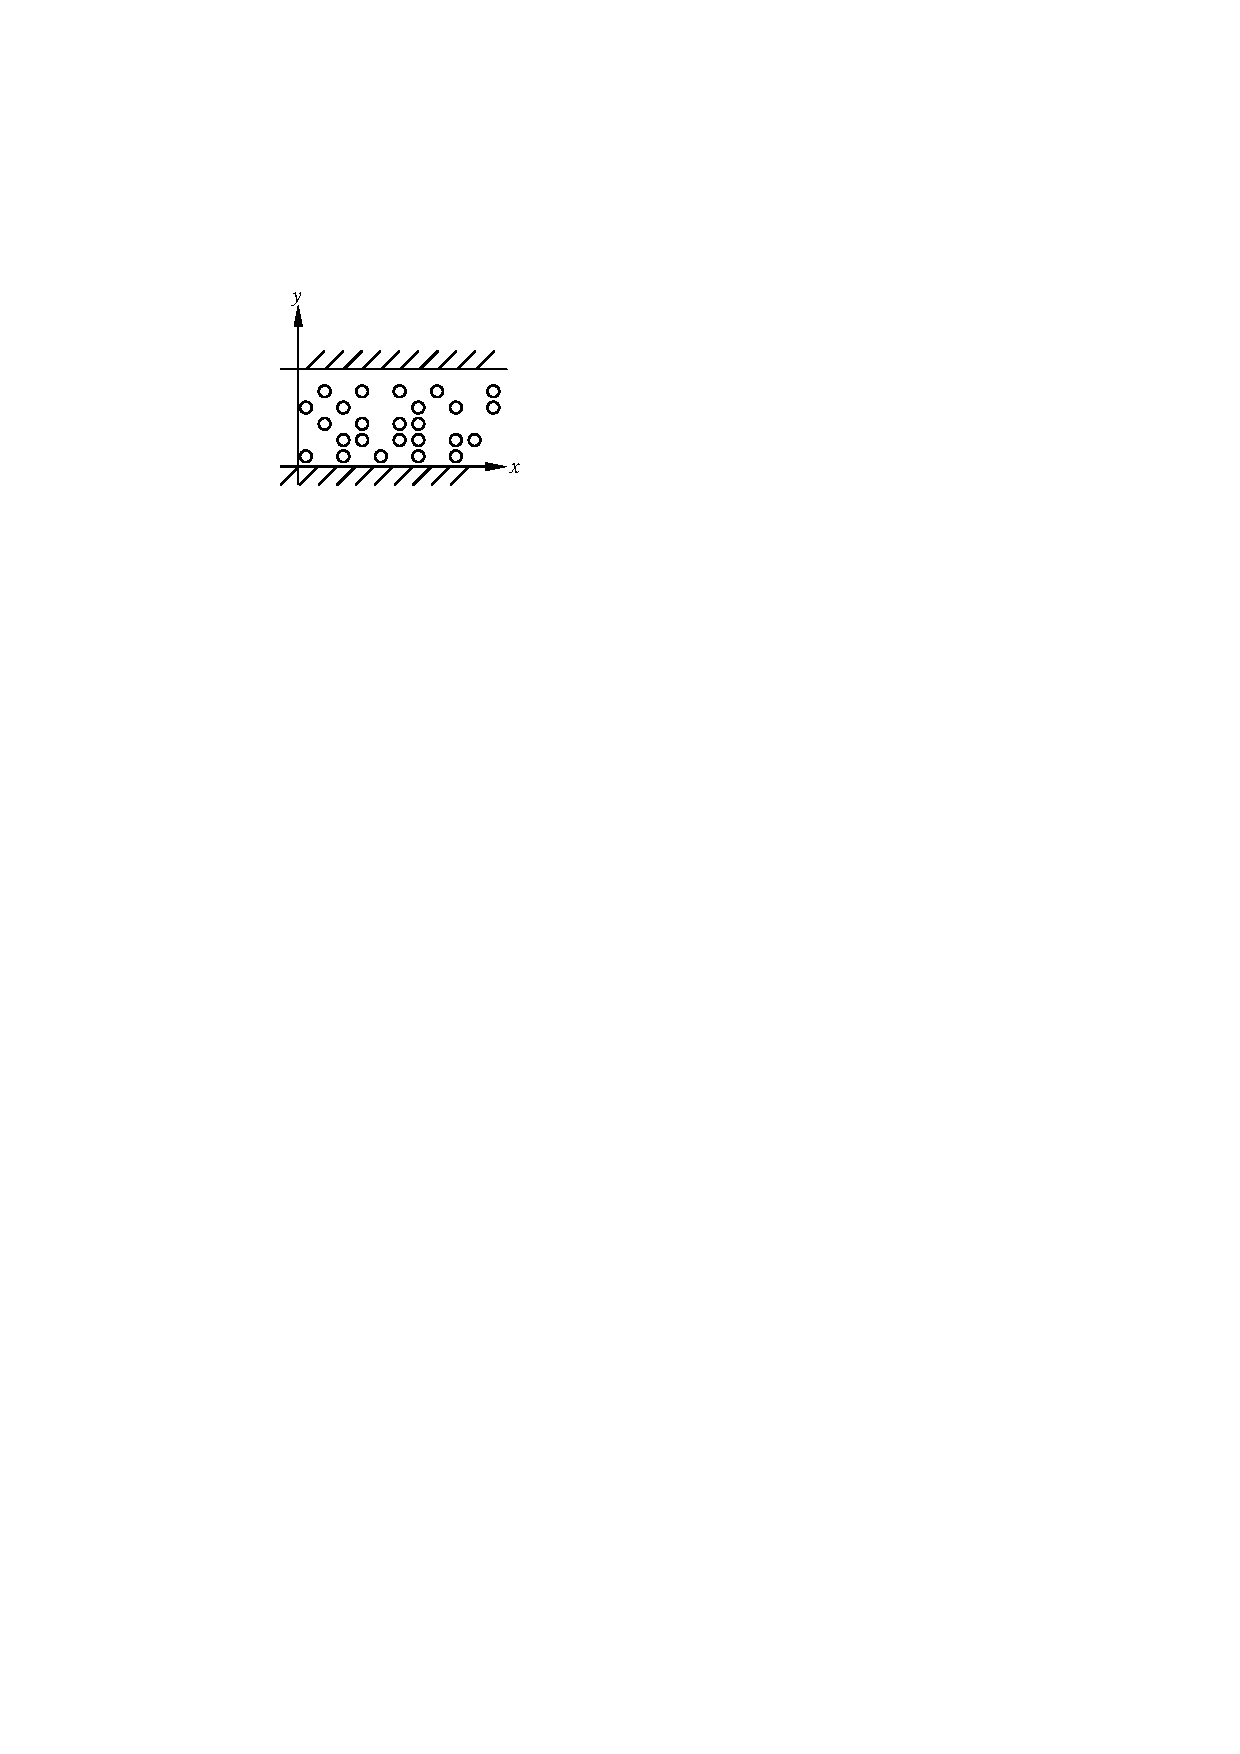
\includegraphics[width=1\textwidth]{./figures/fig04.pdf}

这篇文章对上图的模型分别对反弹映像的三种边界条件作了研究.
\end{column}
\begin{column}[c]{0.6\textwidth}

Dimensionless friction coefficient:
\[
\tau = \gamma\lambda/dv_T
\]

$\gamma$: friction coefficient. $\lambda$: average distance between particles. $d$: spatial dimension(=2). $v_T=\sqrt{k_bT/m}$

The two components of temperature:
\[
T^x = \sum_im_iv_{x_i}^2
,T^y = \sum_im_iv_{y_i}^2
\]
\end{column}
\end{columns}
}

\subsection{结果}
\frame{\frametitle{结果}

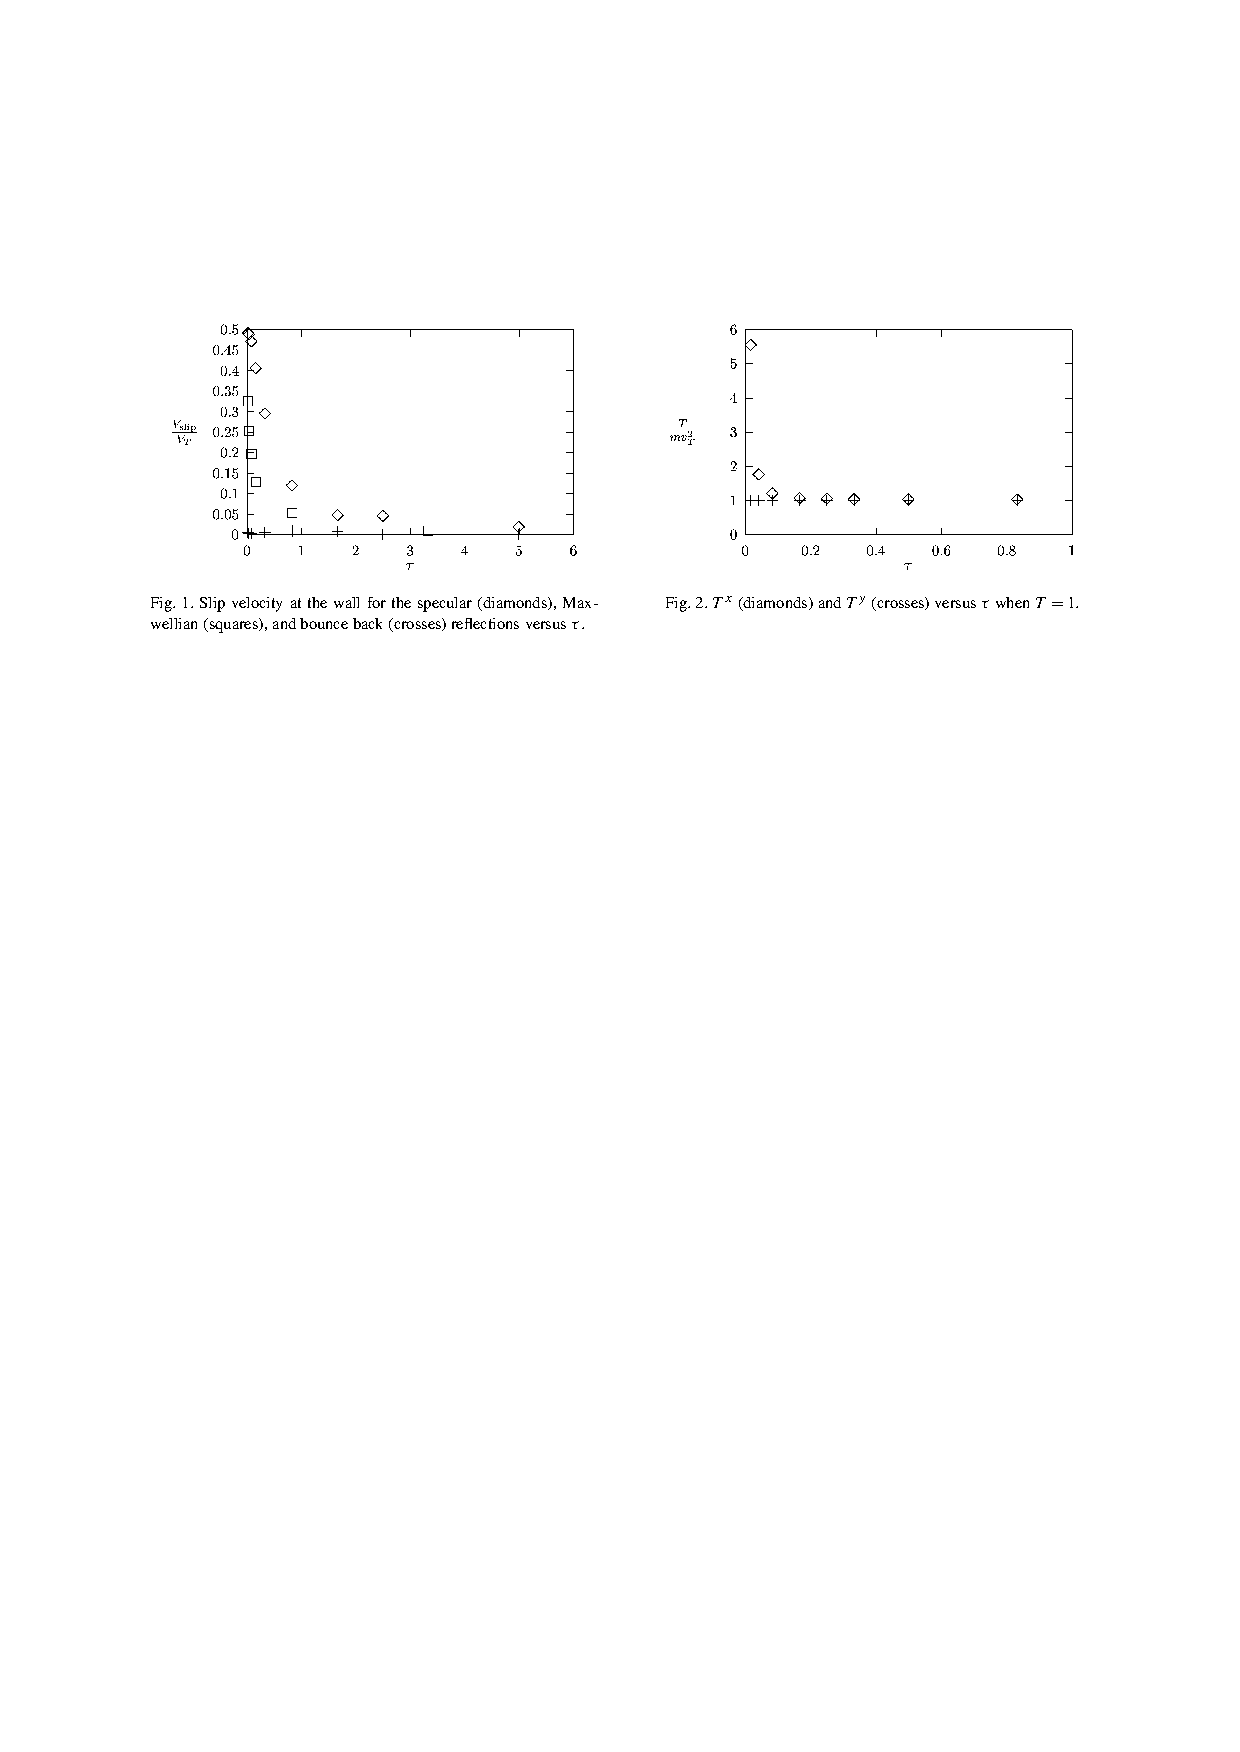
\includegraphics[width=1\textwidth]{./figures/fig05.pdf}
}



\section{A new wall boundary condition in particle methods}

\subsection{模型}
\frame{\frametitle{模型}
\begin{columns}
\begin{column}[c]{0.5\textwidth}
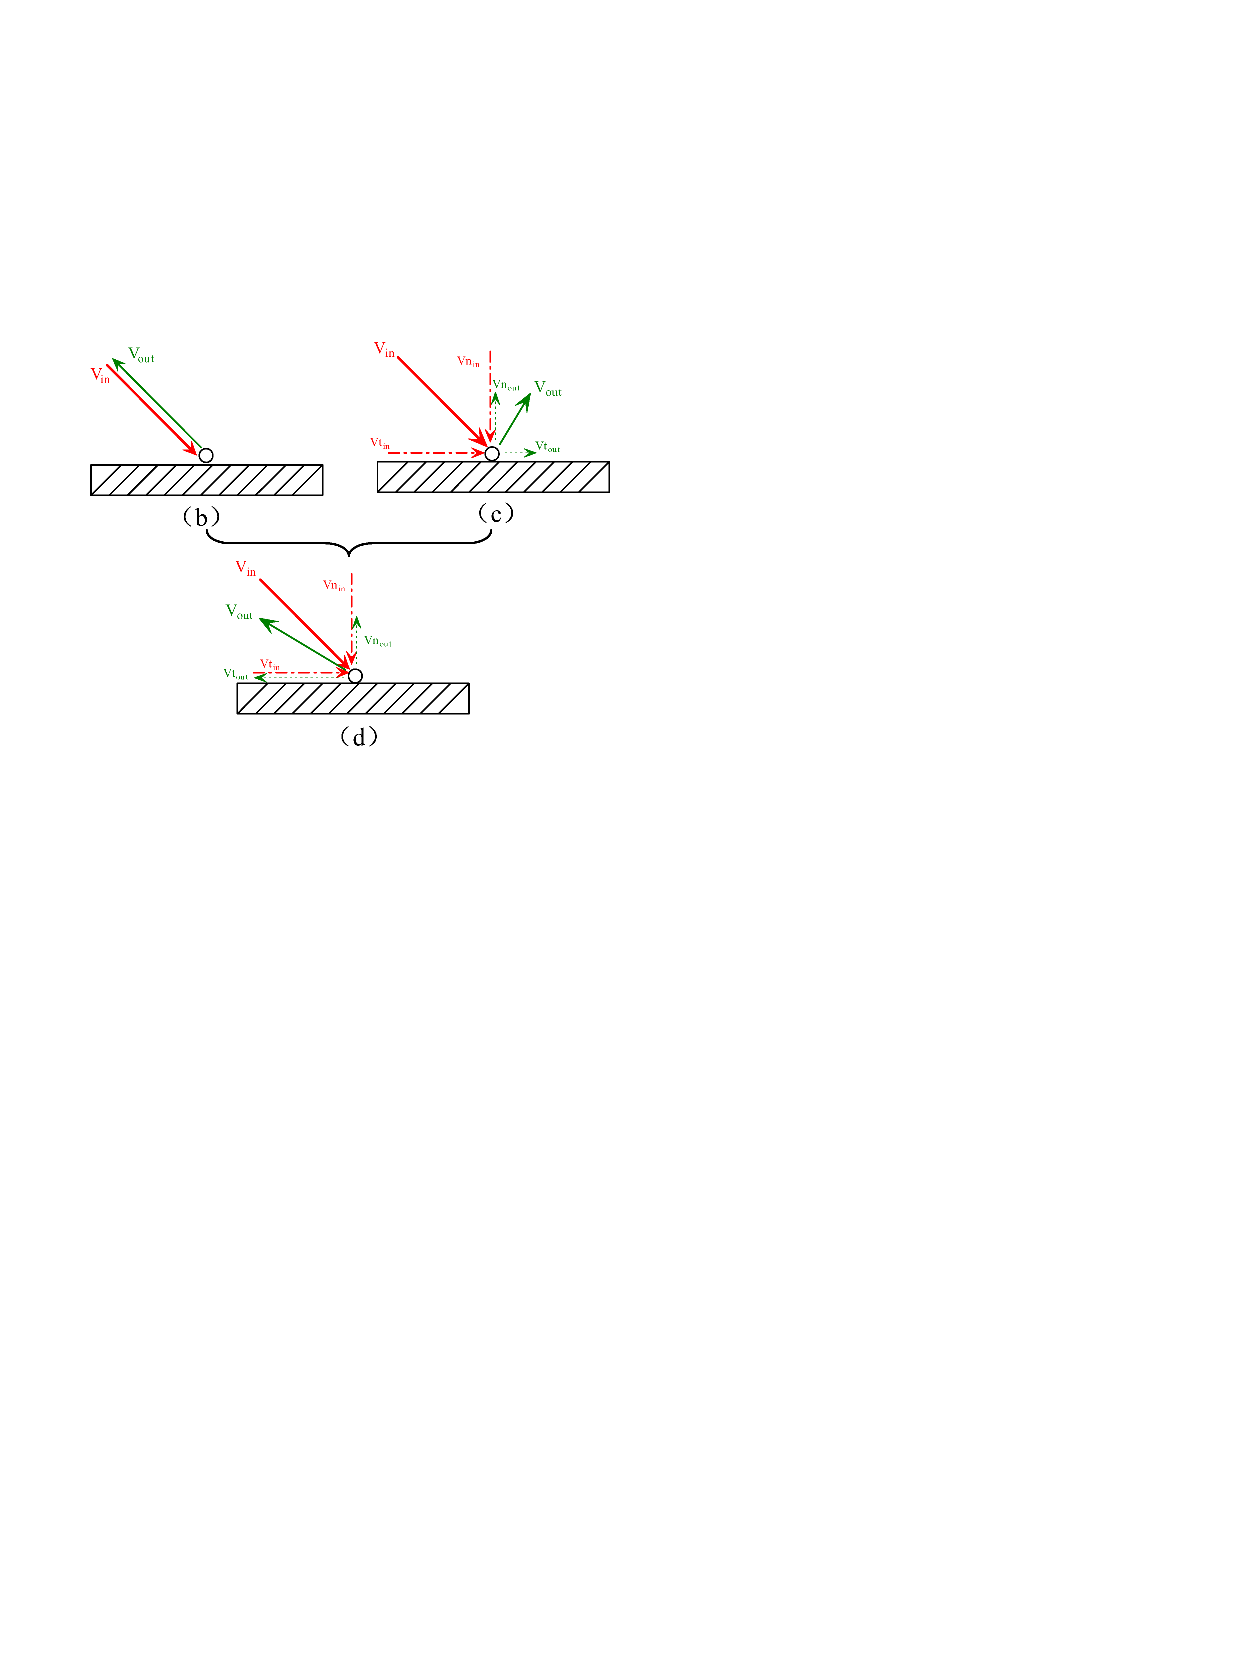
\includegraphics[width=1\textwidth]{./figures/fig06.pdf}
\end{column}
\begin{column}[c]{0.5\textwidth}
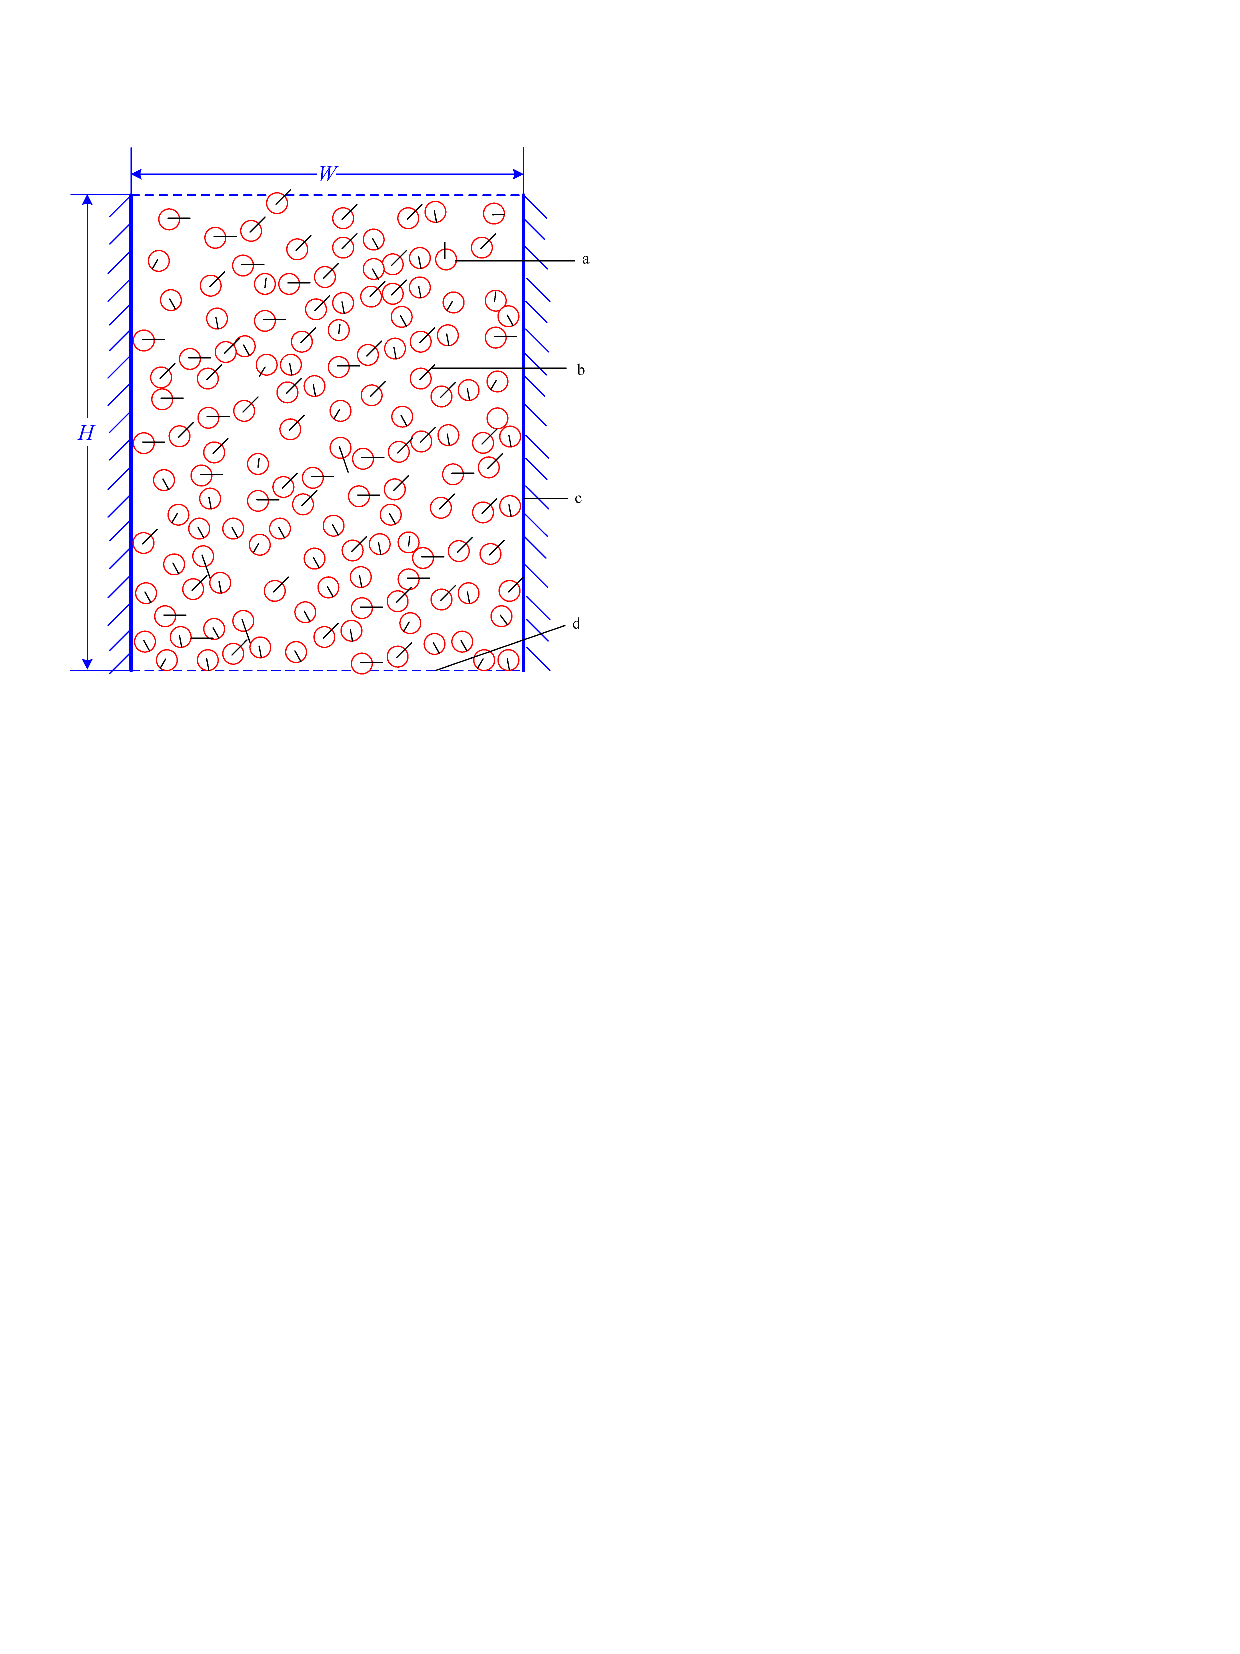
\includegraphics[width=1\textwidth]{./figures/fig07.pdf}
\end{column}
\end{columns}
}

\frame{\frametitle{模型}
与边界作用前后速度分别为
\[
V = v_n\mathbf{n}+v_t\mathbf{\tau}
,
V' = -[(1-\alpha)v_n+\alpha u]\mathbf{n}-v_t\mathbf{\tau}
\]
其中$u$服从
\[
F(u)=2\beta^2u\exp(-\beta^2u^2)
,
 \beta = (2k_b/mT_w)^{-1/2}
\]

Pseudo-particle modeling(PPM): 粒子与粒子作用前后速度$v_1$,$v_{10}$
\[
v_1 = v_{10}-\frac{2m_2}{m_1+m_2}\cdot\frac{(v_{10}-v_{20})\cdot(P_1-P_2)}{|P_1-P2|^2}(P_1-P_2)
\]

}

\subsection{结果}
\frame{\frametitle{两边界的温度相等的结果}
\begin{columns}
\begin{column}[c]{0.5\textwidth}
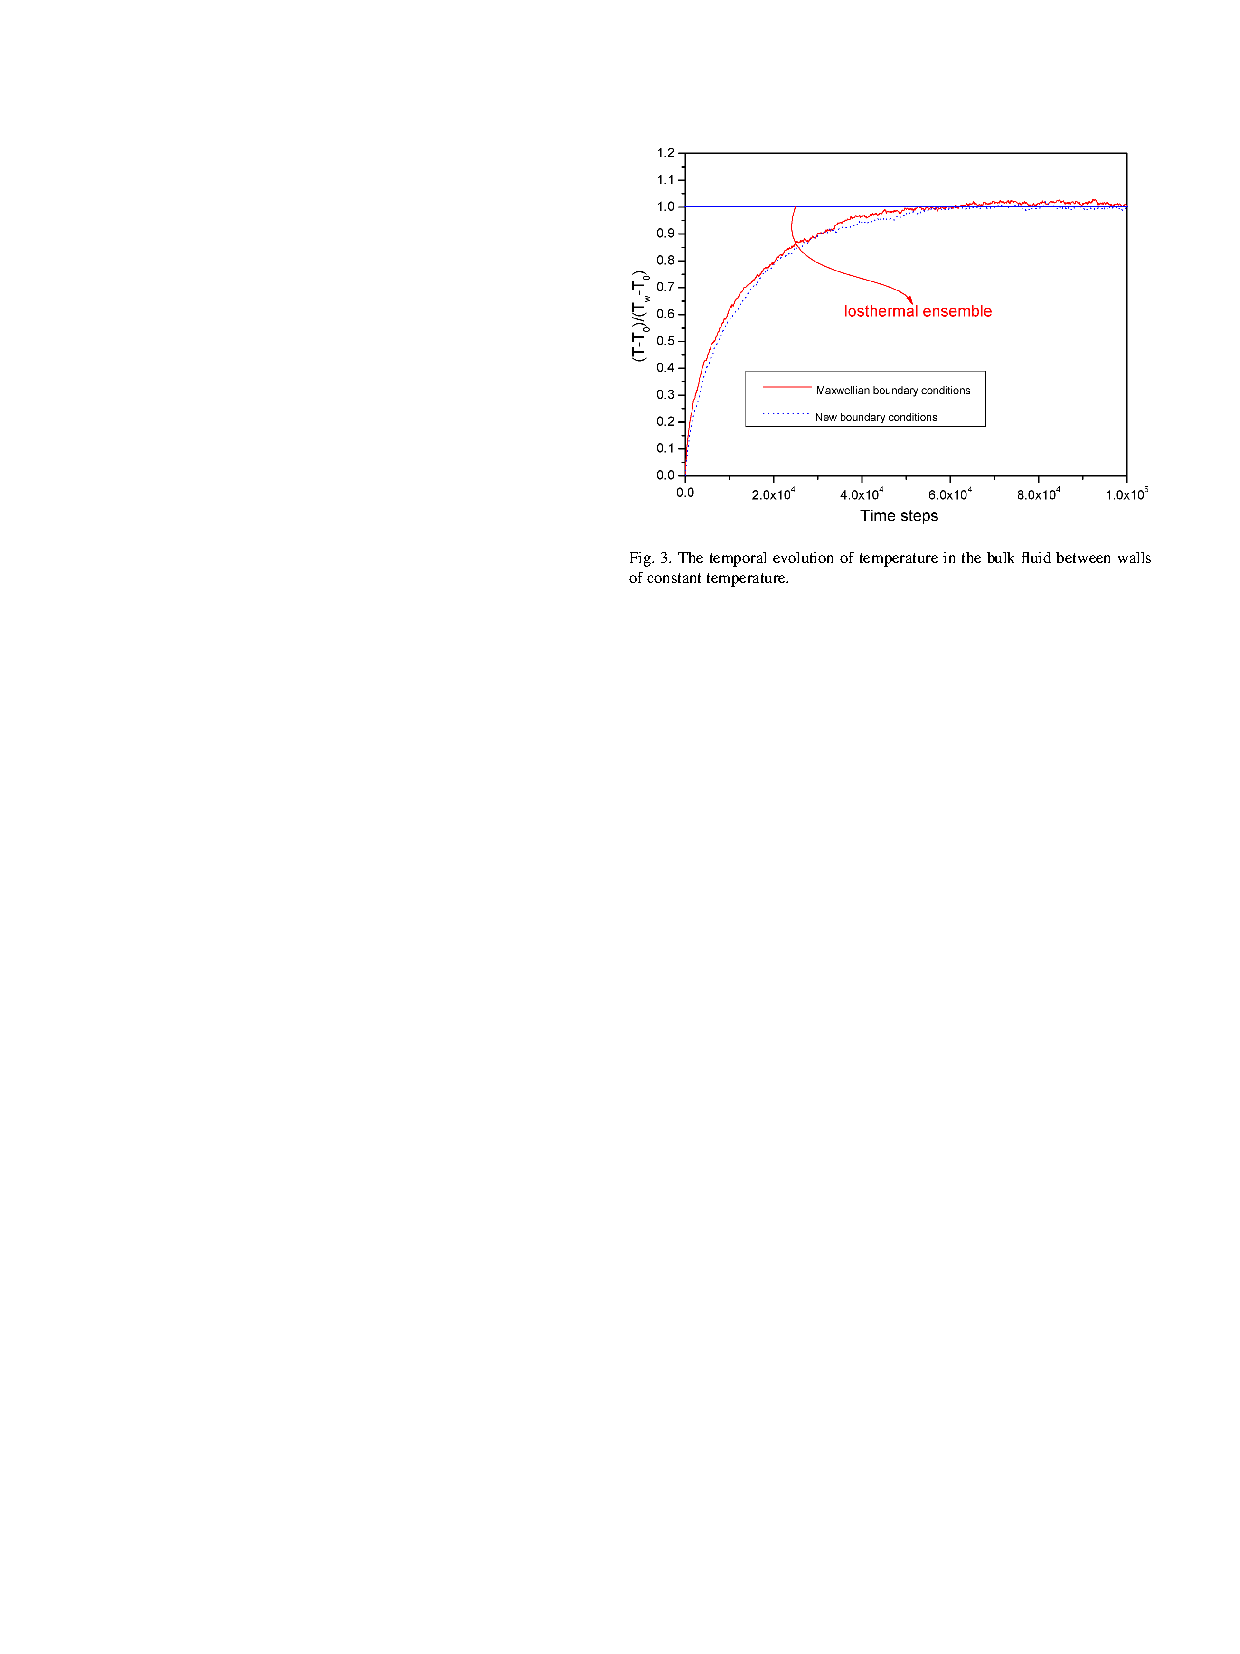
\includegraphics[width=1\textwidth]{./figures/fig08.pdf}
\end{column}
\begin{column}[c]{0.5\textwidth}
两边界的温度相等
\[
T_1=\frac{mv_1^2}{2k_b}=T_2=\frac{mv_2^2}{2k_b}>T_0
\]
\end{column}
\end{columns}
}


\frame{\frametitle{两边界的温度不等的结果}
\begin{columns}
\begin{column}[c]{0.5\textwidth}
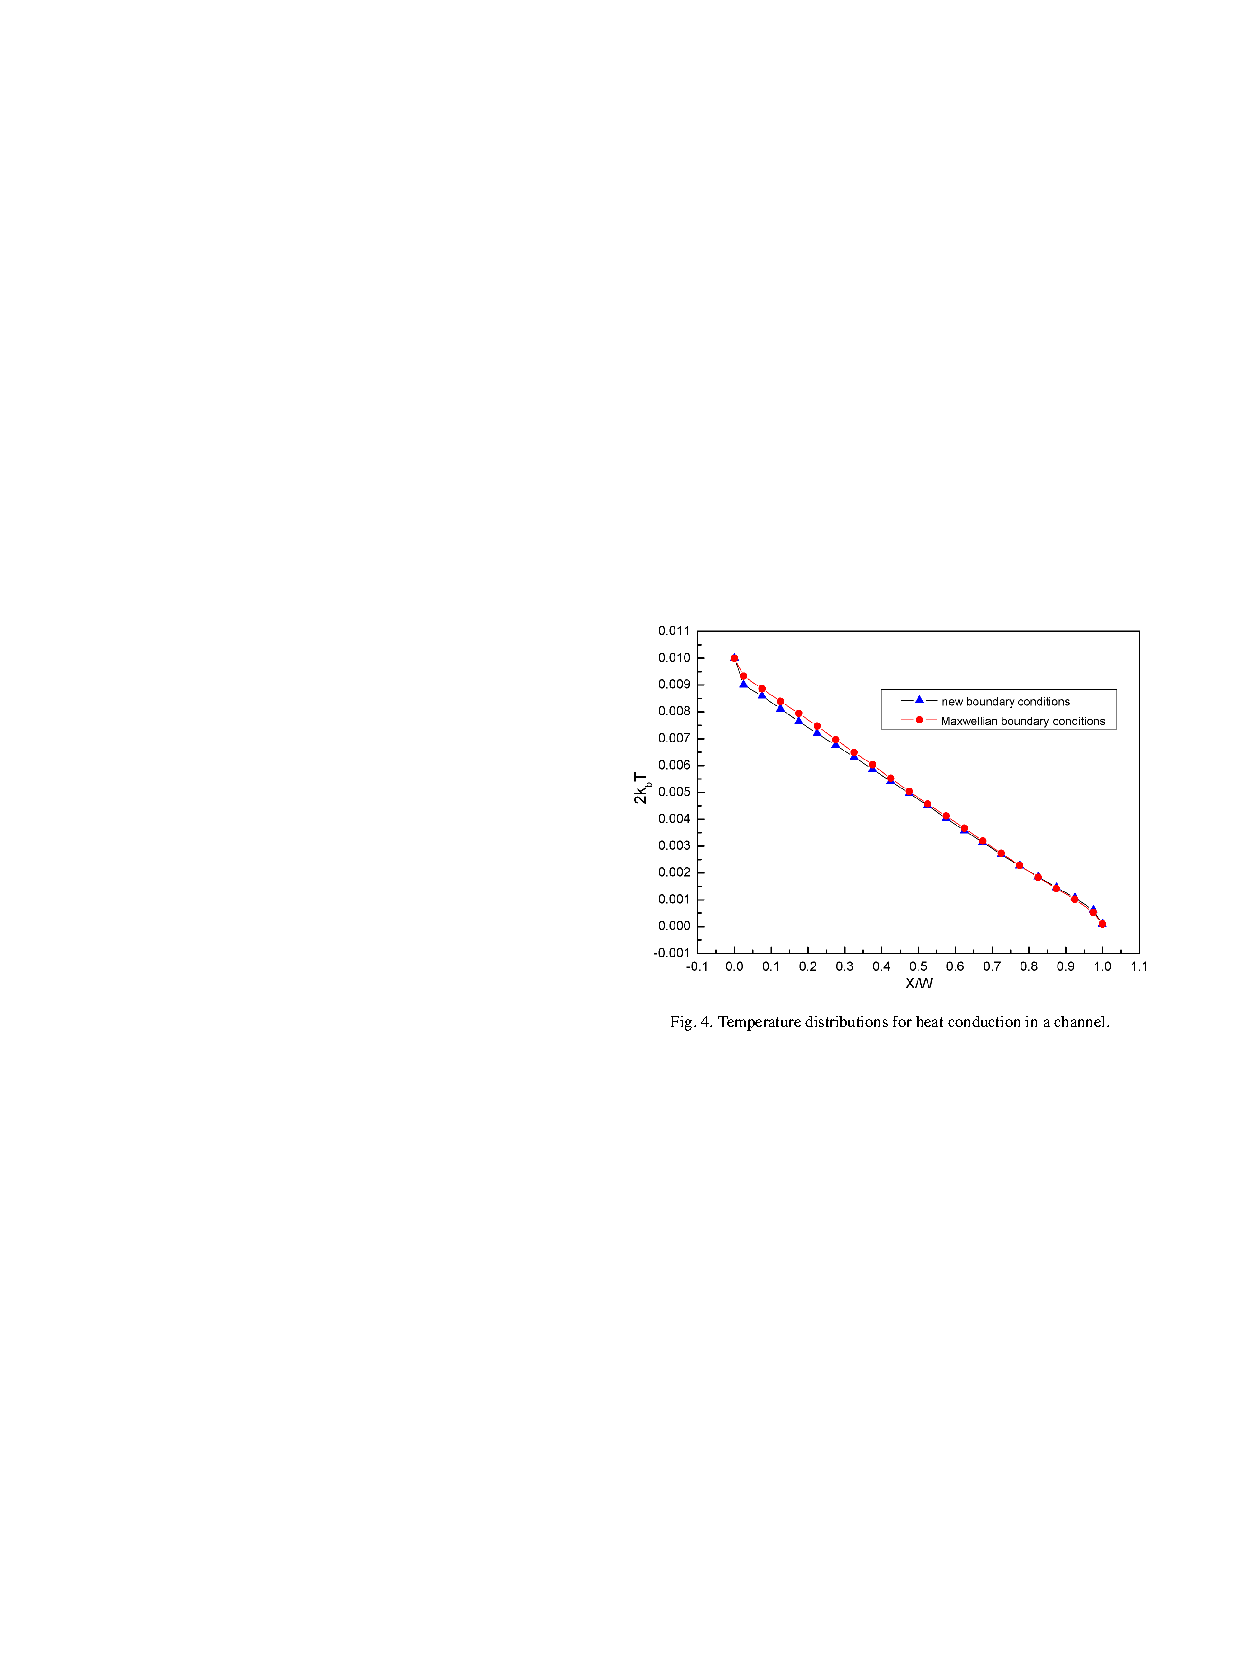
\includegraphics[width=1\textwidth]{./figures/fig09.pdf}
\end{column}
\begin{column}[c]{0.5\textwidth}
两边界的温度不等
\[
T_1=\frac{mv_1^2}{2k_b}>T_0>T_2=\frac{mv_2^2}{2k_b}
\]
\end{column}
\end{columns}
}

\frame{\frametitle{加重力场的结果}
\begin{center}
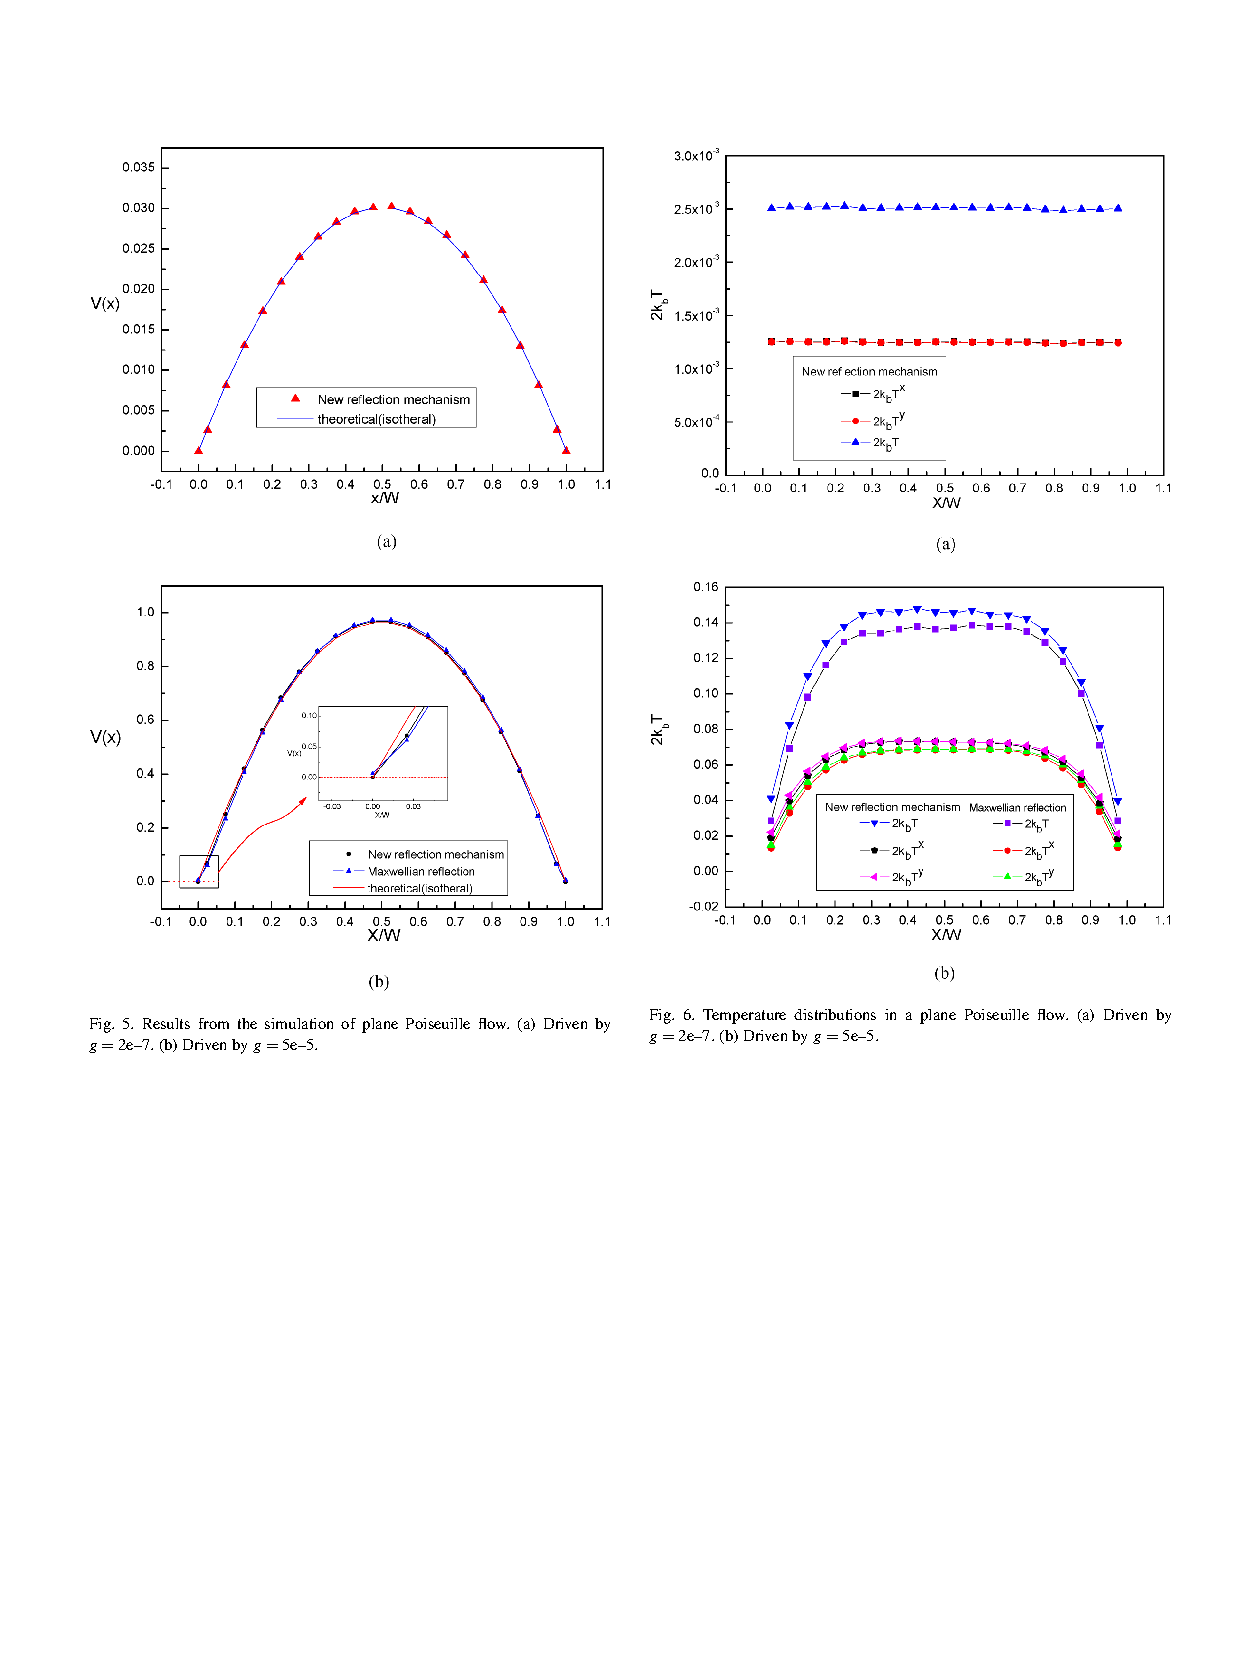
\includegraphics[width=0.77\textwidth]{./figures/fig10.pdf}
\end{center}
}


\section{An implementation of no-slip boundary conditions in DPD}
\subsection{模型}
\frame{\frametitle{模型}
\begin{columns}
\begin{column}[c]{0.5\textwidth}
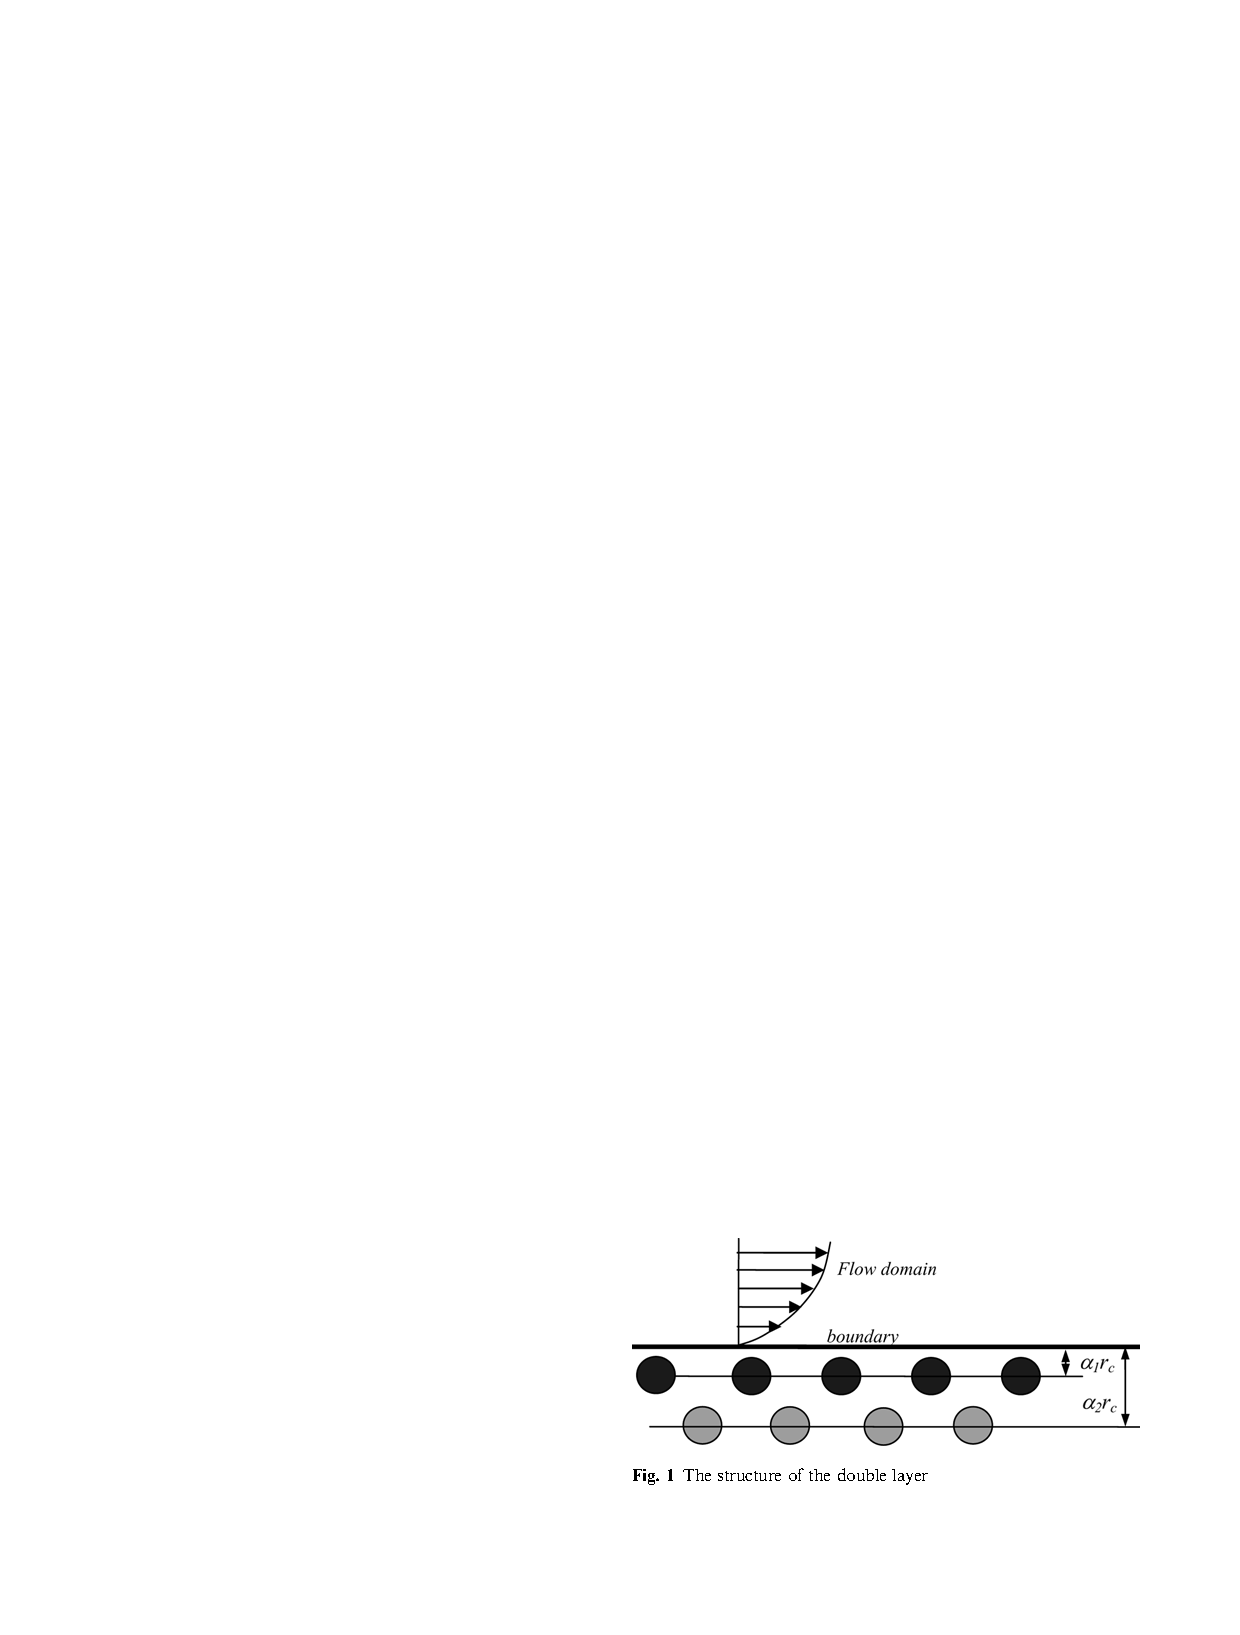
\includegraphics[width=1\textwidth]{./figures/fig11.pdf}
\end{column}
\begin{column}[c]{0.5\textwidth}
$\alpha_1$,$\alpha_2$满足:
\[
0<\alpha_1<\alpha_2
\]

穿过边界的粒子
\[
v_{new} = 2v_{wall} - v_{old}
\]
\[
r_{new} = r_{old} + 2d_r\mathbf{n_w}
\]
\end{column}
\end{columns}
}

\subsection{结果}
\frame{\frametitle{边界单粒子层}
\begin{center}
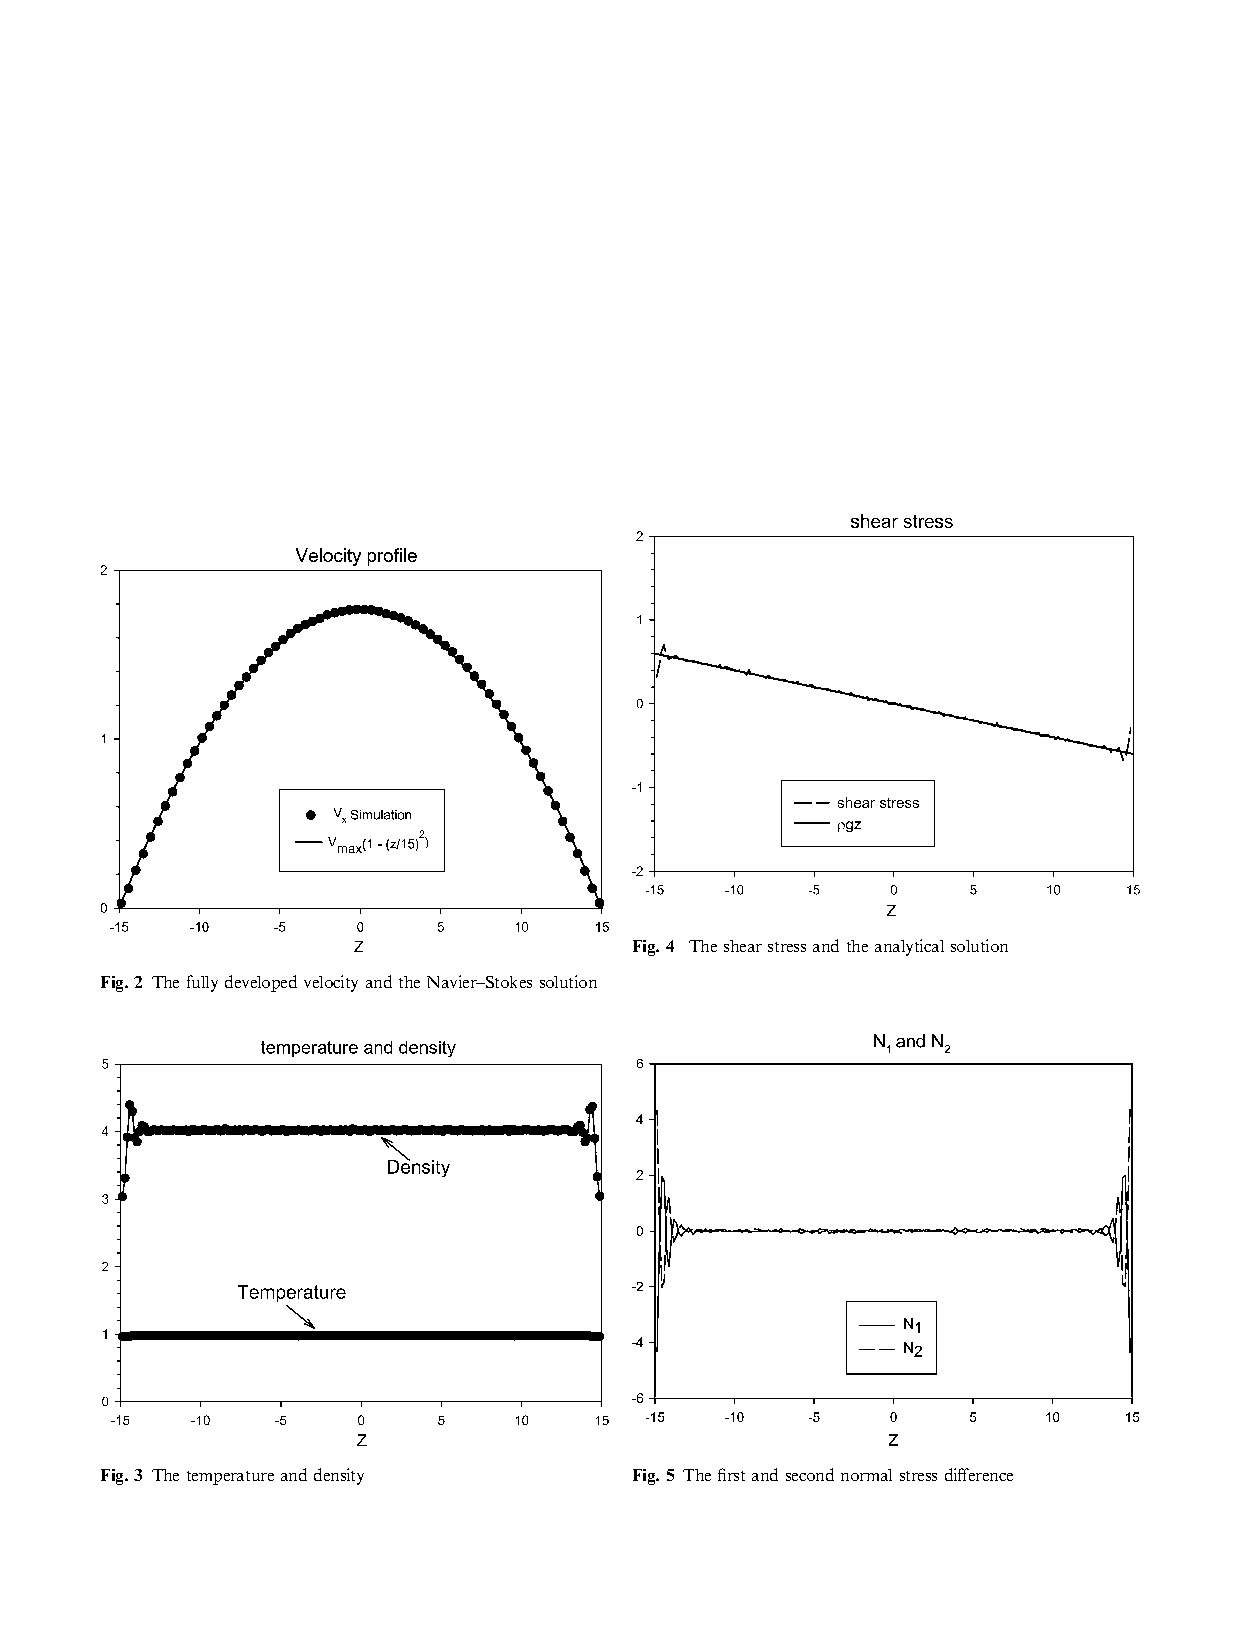
\includegraphics[width=0.7\textwidth]{./figures/fig12.pdf}
\end{center}
}

\frame{\frametitle{边界双粒子层}
\begin{columns}
\begin{column}[c]{0.5\textwidth}
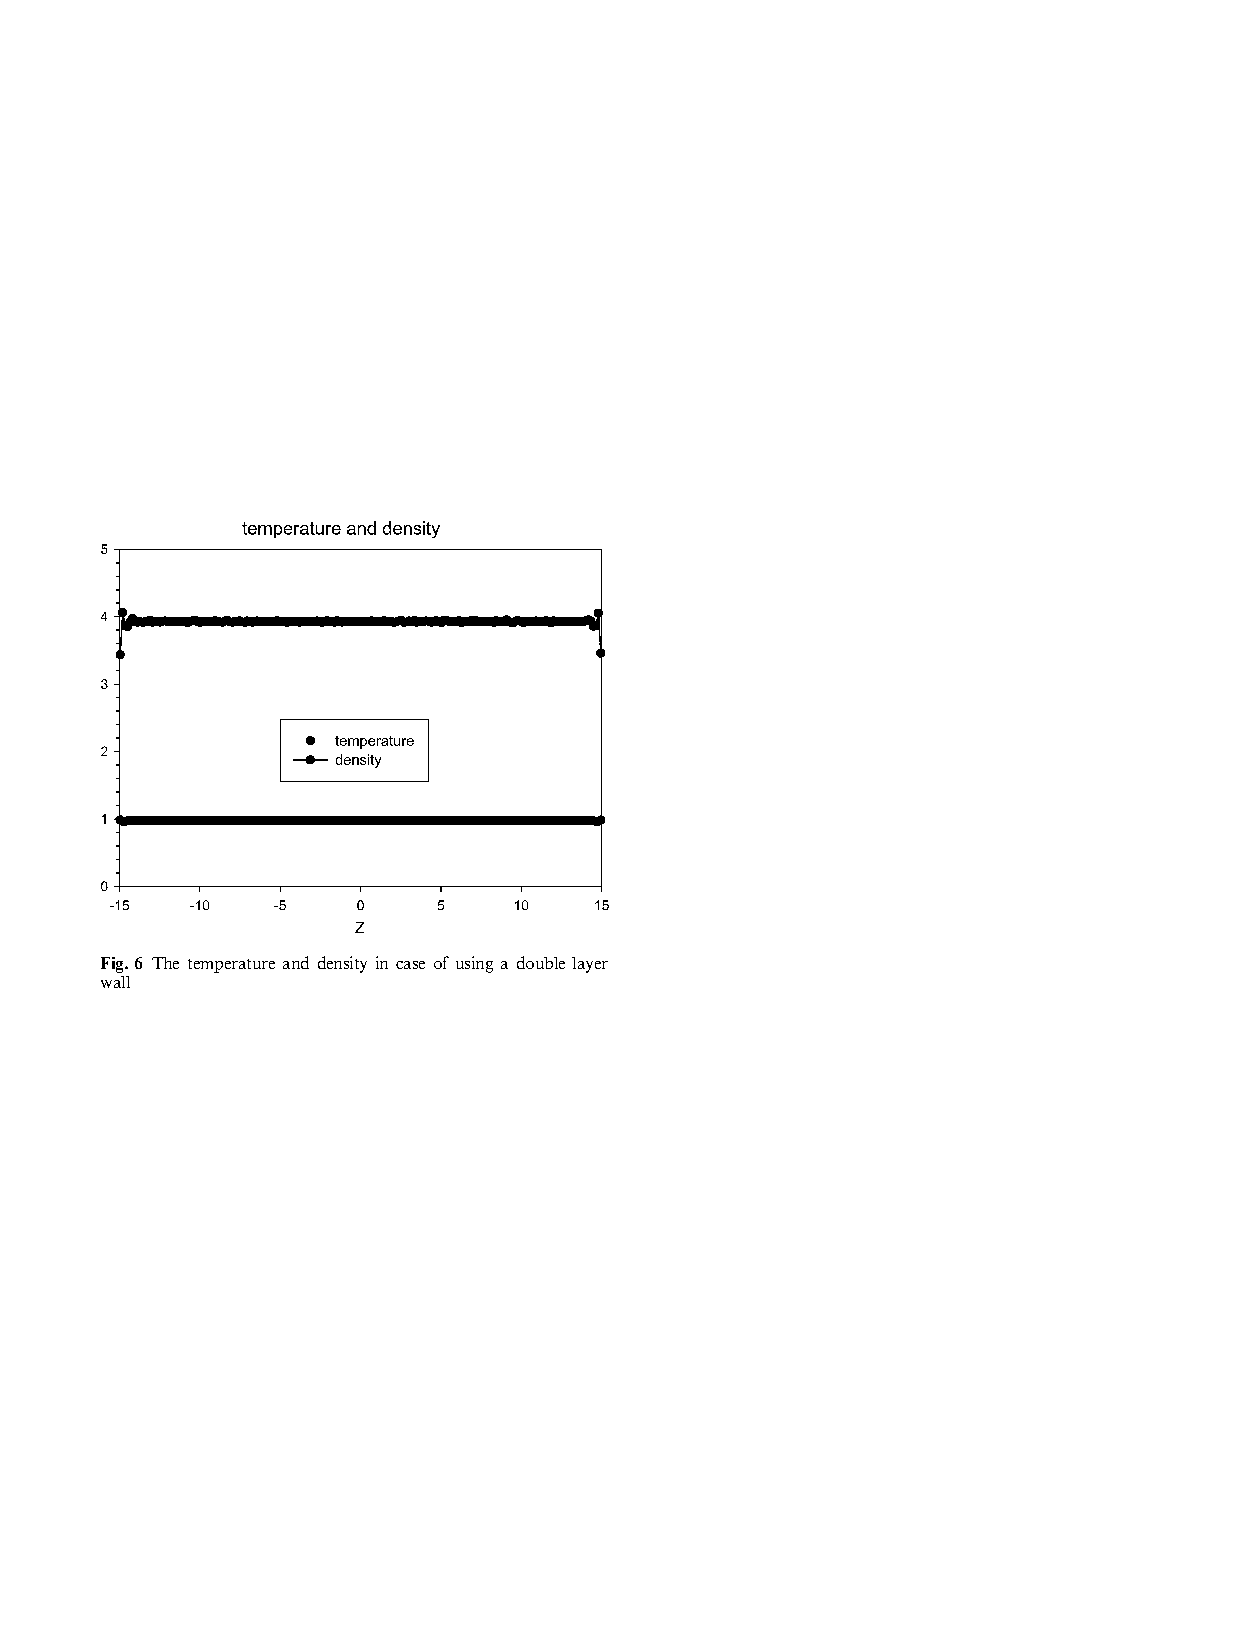
\includegraphics[width=1\textwidth]{./figures/fig13.pdf}
\end{column}
\begin{column}[c]{0.5\textwidth}
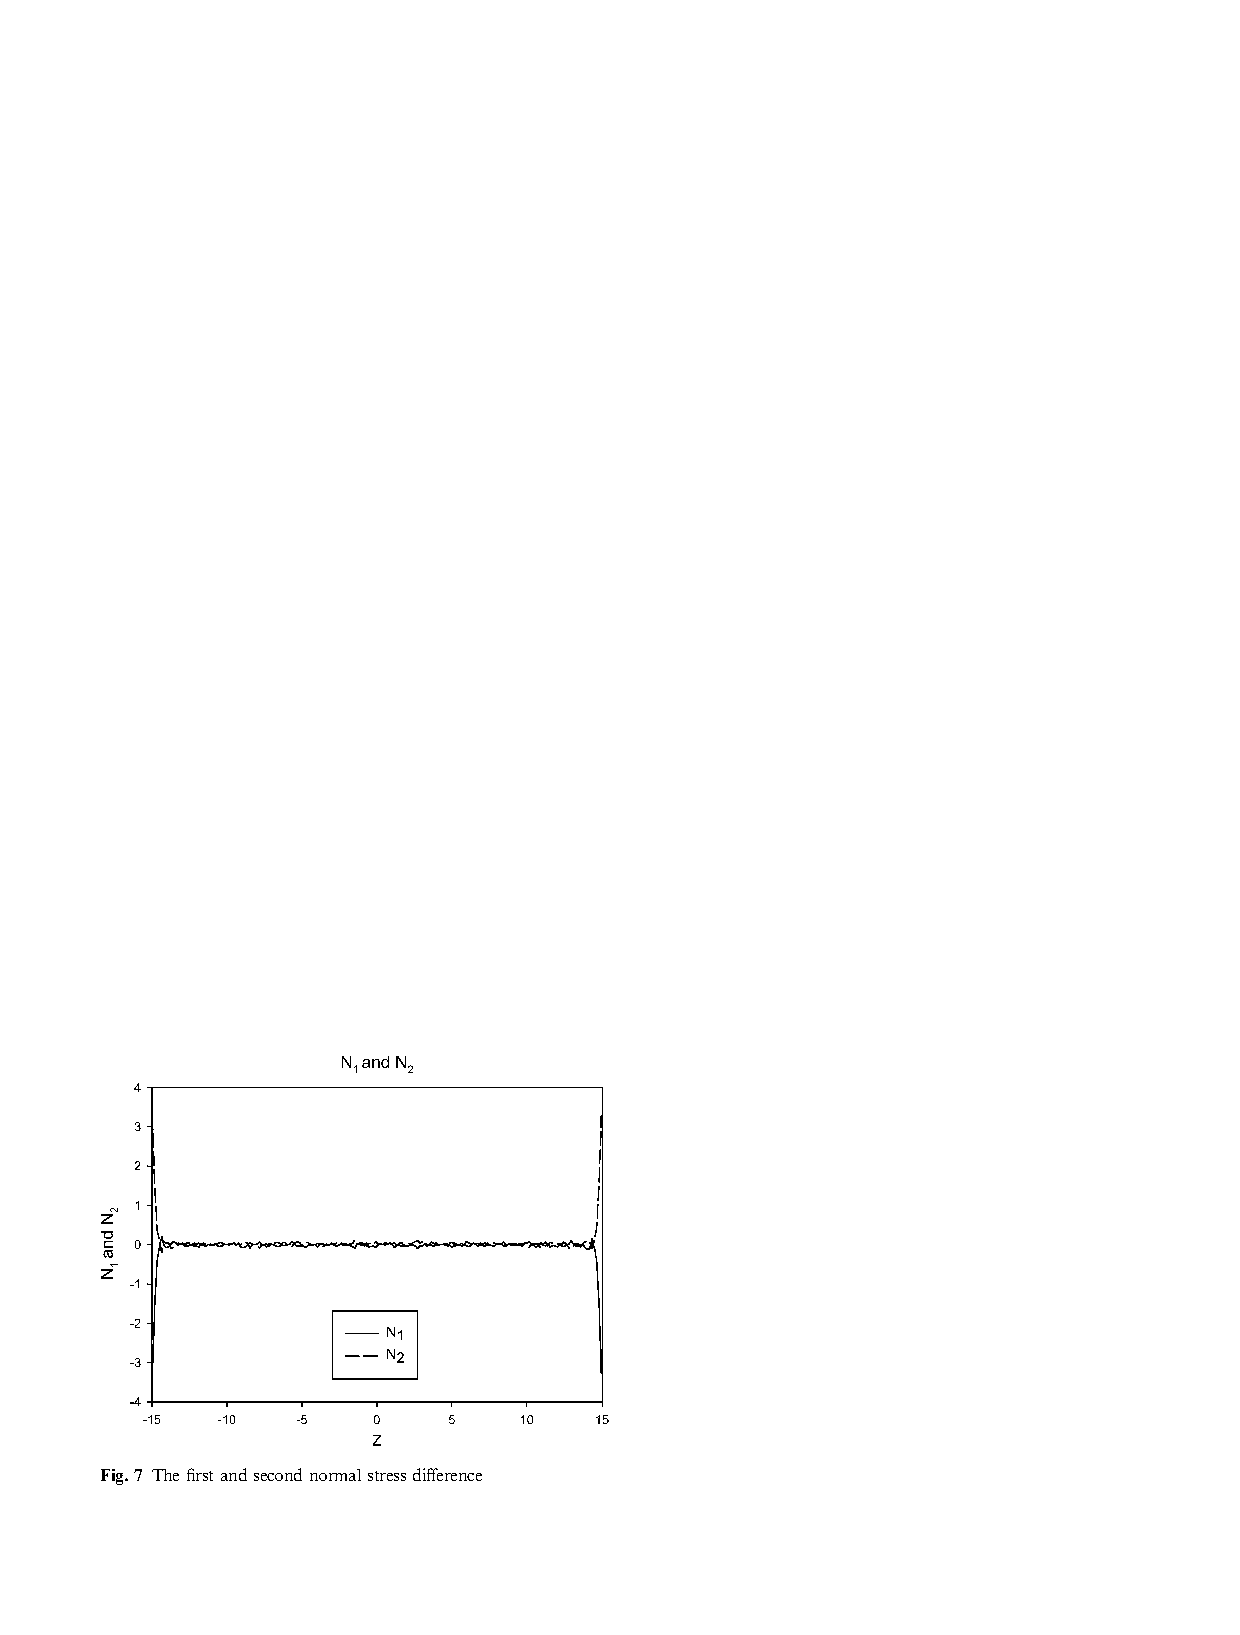
\includegraphics[width=1\textwidth]{./figures/fig14.pdf}
\end{column}
\end{columns}
}


\newcount\opaqueness
\plainframe{
    \begin{centering}
      \Huge Thank You!!!\par
    \end{centering}
} 


\end{document}
